\documentclass[parskip=half, a4paper,twoside,final]{article}
%----Eingebundene Bibliotheken-----
\usepackage[ngerman]{babel}         % Deutsches Sprachpaket
\usepackage[utf8]{inputenc}         % Eingaben codieren
\usepackage[T1]{fontenc}            % Umlaute codieren, Silbentrennung
\usepackage{amsmath, amssymb}       % Mathe
\usepackage{amsthm,amstext,amsxtra} % Symbole für Mathe
\usepackage{mathtools}              % \Aboxed Boxen in align
\usepackage{wrapfig}                % Bilder umfließen
\usepackage{svg}                    % Vektorgraphiken einbinden
\usepackage{geometry}               % Papierformat
\usepackage{tabularx}               % Tabellen
\usepackage{xcolor,colortbl}        % Farben
\usepackage{graphicx}               % Für Limes Definition wichtig
\usepackage{soul}                   % Unterstreichungen
\usepackage[section]{placeins}      % \Floatbarrier
\usepackage{wrapfig}                % Bilder umfließen
\usepackage{enumerate}              % Aufzählungen
\usepackage{footnote}               % Fußzeilen
\usepackage{booktabs}               % publication quality tables
\usepackage[hyphens]{url}           % \url{}
\usepackage{bm}                     % bold symbols \bm{r}
\usepackage{dsfont}                 % identity matrix \mathds{1}
\usepackage{enumitem}               % itemize Umgebungen customizen
\usepackage{esint}                  % Doppelintegrale
\usepackage{fancyhdr}               % schöne Kopf- und Fußzeilen
\usepackage{lmodern}
\usepackage{tikz}
\usepackage{pgfmath, pgfplots}
\usepackage[labelfont=bf]{subcaption}
\usepackage[square,numbers,sort&compress]{natbib}
\usepackage{mhchem}                 % Chemistry Package
\usepackage{physics}
\usepackage{chemfig}
\usepackage[detect-all,
            locale=DE,binary-units,
            exponent-product=\cdot
            ]{siunitx}              % \SI{12}{\gram}
%siunitx stellt für Tabellen den Spaltentyp S bereit ==> Ausrichtung an Dezimaltrennzeichen
\usepackage[position=below,
            tableposition=top,
            format=hang,
            labelfont=it,
            labelfont=bf,
            ]{caption}              % Settings für Captions
\captionsetup[wrapfigure]{name=Abb.}
\usepackage[europeanvoltages,
            europeancurrents,
            europeanresistors,
            americaninductors,
            europeanports
            ]{circuitikz}           % Schaltungen
\usepackage{chngcntr}               % vor hyperref laden!
  \counterwithin*{equation}{section}
  \counterwithin*{figure}{section}
  \counterwithin*{table}{section}

\usepackage[final,
            pdfauthor={Martin Beyer, Vanessa Huth},
            pdfsubject={Fortgeschrittenen-Praktikum},
            pdffitwindow=true,      % resize document window
            pdftitle={Fortgeschrittenen-Praktikum},
            bookmarks=true,         % lesezeichen-Liste
            bookmarksopen=true,     % Lesezeichen geöffnet
            bookmarksopenlevel=1,
            bookmarksnumbered=true,
            colorlinks=true,        % fuer Druckversion auf "false"
            linkcolor=blue,         % Table of Contents, Footnotes
            urlcolor=blue,          % fuer eingebunden URLs
            citecolor=blue,         % Equations, References
            filecolor=blue,
            pdfborder={0 0 0},      % keine Rahmen um Links: {0 0 0}
            ]{hyperref}


% Commands
\renewcommand{\sfdefault}{lmss}     % latin modern sans serif
\newcommand{\R}{\mathbb{R}}         % Reelle Zahlen
\newcommand{\N}{\mathbb{N}}         % Natürliche Zahlen
\newcommand{\C}{\mathbb{C}}         % Komplexe Zahlen
\newcommand{\de}{\mathrm{d}}      % Differential
\newcommand{\entspricht}{\mathrel{\widehat{=}}}

\DeclareSIUnit{\eV}{\text{eV}}
\DeclareSIUnit{\voltpeakpeak}{\volt{\textsubscript{pp}}}

% Dokumenteneinstellungen
\setlength{\parindent}{0px}         % remove indent in new paragraph
\setlength{\parindent}{0px}         % keine Absätze durch Leerzeilen im Code
\emergencystretch=1em % Definiert den Leerraum, der innerhalb einer Zeile zusätzlich verteilt werden darf.
\setlength{\topmargin}{-5mm} % 210mm = 8.2677165in
\newlength{\mylength}
\setlength{\mylength}{\paperwidth}
\addtolength{\mylength}{-2in} % standardmäßig wird den Seitenrändern jeweils noch 1in = 25.4mm hinzuaddiert
\setlength{\textwidth}{145mm}
\setlength{\textheight}{230mm}
\addtolength{\mylength}{-\textwidth}
\setlength{\oddsidemargin}{10mm}
\addtolength{\mylength}{-\oddsidemargin}
\setlength{\evensidemargin}{\mylength}
\setlength{\marginparwidth}{1.7cm}
\interfootnotelinepenalty=10000

% Umdefinition von \textcolor ********************************************************
\makeatletter
\renewcommand*{\@textcolor}[3]{%
	\protect\leavevmode
	\begingroup
	\color#1{#2}#3%
	\endgroup
}
\makeatother
% Damit das auch im Mathemodus anwendbar ist und dort z.B. die Leerzeichen nicht wie im Textmodus gesetzt werden.

\pgfplotsset
{compat=newest, % aktuelle Version: 1.16 [29.05.2018]
	/pgf/number format/.cd, % cd steht fuer current directory
	%  	use comma, % Komma als Dezimaltrennzeichen %%% UNCOMMENT THIS !!!
	1000 sep={} % Legt das Tausendertrennzeichen fest
}
%\usepgfplotslibrary{external} % Section 7.1.1 Using the Automatic Externalization Framework of TikZ
%\tikzexternalize[prefix=FiguresTikZ/] % activate externalization! Use subdirectory [FiguresTikZ]
\usepgfplotslibrary{fillbetween}
\usepgfplotslibrary{polar}
\usetikzlibrary{arrows.meta}
\usetikzlibrary{calc}
\usetikzlibrary{datavisualization.formats.functions}
\usetikzlibrary{intersections}
\usetikzlibrary{patterns}
\usetikzlibrary{pgfplots.colormaps}
\usetikzlibrary{plotmarks}
\usetikzlibrary{shapes.geometric}

% Generelle Festlegung des Styles fuer Blockschemata (Plaene fuer Regelkreise, etc.)
\tikzstyle{block} = [draw, fill=blue!20, rectangle, minimum height=1cm, minimum width=1cm]%, minimum width=6em]
\tikzstyle{sum} = [draw, fill=blue!20, circle, node distance=1cm]
\tikzstyle{input} = [coordinate]
\tikzstyle{output} = [coordinate]
\tikzstyle{pinstyle} = [pin edge={to-,thin,black}]


\begin{document}
\setlength{\marginparsep}{2em}
\renewcommand{\theequation}{\arabic{section}.\arabic{equation}}
\renewcommand{\thefigure}{\arabic{section}.\arabic{figure}}
\renewcommand{\thetable}{\arabic{section}.\arabic{table}}

% Anfang ********************************************************
\begin{center}
\thispagestyle{empty}
  
\includegraphics[width=0.75\textwidth]{../UniJena_BildWortMarke_black.pdf}\\[4em]
  \Large
  Ausarbeitung zum Versuch\\[2em]
  \Huge
  Festkörpereigenschaften bei tiefen Temperaturen\\
  \vspace{2cm}
  \Large
  Martin Beyer und Vanessa Huth\\[2em]
  Abgabe: 30. September 2020\\[2em]
  Betreuer: Matthias Thürk\\[5em]
  \begin{flushleft}
  	Bewertung und Ausarbeitung:\\[2em]
		Protokollführung und Form:\\[1em]
		Ergebnisse, Auswertung und Interpretation:\\[1em]
		Bemerkungen und Hinweise des Betreuers:
  \end{flushleft}
\end{center}
\clearpage

\pagestyle{fancy}
\renewcommand{\headrulewidth}{0pt}
\renewcommand{\footrulewidth}{0.5pt}
\renewcommand{\sectionmark}[1]{\markright{#1}}
\fancyhead[RO,LE]{\textbf{Tieftemperatur}}
\fancyhead[RE,LO]{\rightmark}
\fancyfoot[LE,RO]{\bfseries\thepage}
\fancyfoot[CO,CE]{Protokoll}
\renewcommand{\headrulewidth}{0.5pt}
\renewcommand{\footrulewidth}{0.5pt}

\setcounter{equation}{0}
\setcounter{figure}{0}

% *********************************************
% ***** KAPITEL 1 *****************************
% *********************************************
\tableofcontents
% \pagenumbering{gobble}% remove page numbering
\newpage
% \pagenumbering{arabic}
\section{Aufgabenstellung} \label{sec:Aufgabenstellung}

\subsection{Aufbau geeigneter Tieftemperaturmesstechnik}

Es werden Widerstandsthermometer Pt 100 und Pt 1000, sowie Siliziumdioden als Sekundärthermometer verwendet. Es soll die Anfangstemperatur an den Sensoren auf folgende Weisen vermessen werden:
\begin{enumerate}
  \item Zweileiterschaltung mit Temperaturmessfunktion des Digitalvoltmeters (DVM), einmal ohne und einmal mit Kompensation des Messleitungswiderstandes.
  \item Zweileiterschaltung mit Konstantstromquelle und Spannungsmessung mit DVM.
  \item Vierleiterschaltung mit Konstantstromquelle und Spannungsmessung mit DVM.
\end{enumerate}

Es werden die Vor- und Nachteile der betrachteten Verfahren diskutiert.

\subsection{Bestimmung des temperaturabhängigen Widerstandes eines Halbleiters}

\begin{enumerate}
  \item Es wird eine Messchaltung zur Bestimmung des temperaturabhängigen Widerstandes und der Temperatur eines Gold-dotierten Germaniumhalbleiters aufgebaut.
  \item Der Abkühlvorgang der Gifford-McMahon Kleinkältemaschine wird aufgenommen.
  \item Es erfolgt eine Bestimmung der wirksamen Bandlücke zwischen Akzeptorniveau und Valenzelektronenband aus dem Verlauf von Widerstand über der Temperatur.
\end{enumerate}
Der relative Widerstand wird logarithmisch als Funktion von $1/T$ aufgetragen und die Wirkung von Dotierungen auf die Halbleitereigenschaften diskutiert.

\subsection{Abkühlverhalten von Proben in kryogenen Flüssigkeiten}
\begin{enumerate}
  \item Es wird das Abkühlverhalten eines Kupferzylinders mit und ohne thermische Isolation untersucht.
  \item Die Abkühlung der beiden Probenkörper in flüssigem Stickstoff wird realisiert.
  \item Die Wärmeübergangszahl $\alpha$ wird für das Blasen- und Filmsieden aus der Energiebilanz des Wärmeübergangs bestimmt.
\end{enumerate}
Es wird die Frage beantwortet, warum die Wärmeübergangszahl $\alpha$ für den thermisch isolierten Körper nicht bestimmt werden kann. Die ermittelten Werte werden mit bekannten Literaturwerten verglichen.

\subsection{Temperaturabhängigkeit der molaren Wärmekapazität fester Stoffe bei kryogenen Temperaturen}

Es wird eine thermische Zyklierung der Probenkörper aus Kupfer und Blei realisiert und die molare Wärmekapazität für jeweils zwei Temperaturbereich bestimmt.



% *********************************************
% ***** KAPITEL 2 *****************************
% *********************************************
\newpage
\section{Grundlagen} \label{sec:Grundlagen}

\subsection{Eigenschaften von Halbleitern}
Für einzelne Atome lassen sich mithilfe der \textsc{Schrödinger}-Gleichung diskrete Energieniveaus für die im Atom befindlichen Elektronen berechnen. Nähern sich zwei Atome einander an, dann verschieben sich die Energieniveaus aufgrund der elektrostatischen Wechselwirkung der vorhandenen Elektronen. Für einen Kristall mit einer Vielzahl an Atomen verschmieren schließlich die Energieniveaus zu sogenannten Energiebändern. Zwischen diesen treten verbotene Zonen elektrischer Zustände der Elektronen auf.

Das höchste, bei $T=\SI{0}{\kelvin}$ besetzte Energieband ist das Valenzband und das darüberliegende energiereichere Band wird Letungsband genannt. Die Energiedifferenz zwischen Leitungsbandunterkante $E_L$ und Valenzbandoberkante $E_V$ ist die Bandlücke $E_g$ und charakterisiert die Eigenschaften des Festkörpers. Je nach Größe der Bandlücke wird zwischen Nicht-, Halbleitern und Leitern unterschieden, wie Abbildung~\ref{fig:Bandschema} zeigt.

\input{Bilder/Bändermodell.tex}

Eine endliche Leitfähigkeit von Halbleitern kann erreicht werden, indem Elektronen die nötige Energie zugeführt wird, um die Bandlücke zu überwinden. Dies kann durch thermische Anregung $E_\text{th} = k_B T$ geschehen, was bei Zimmertemperatur etwas $\SI{25}{\milli\electronvolt}$ sind. Dies reicht nicht aus, um Eigenleitung im typischen Halbleiter zu erzeugen.

Im realen Halbleiter treten immer Verunreinigungen durch Fremdatome auf, die die Leitfähigkeit erhöhen. Oft wird dieser Effekt gezielt durch das Einbringen Dotieratomen genutzt. Das Dotieratome verdrängt dabei ein Atom aus dem Kristallgitter. Es lässt sich zwischen zwei Arten unterscheiden:
\begin{enumerate}
  \item p-Dotierung: Ein Atom mit weniger Valenzelektronen wird eingebracht. Es entsteht ein Elektronenloch, was durch benachbarte Elektronen besetzt werden kann und einen Stromfluss erzeugt.
  \item n-Dotierung: Ein Atom mit mehr Valenzelektronen wird eingebracht. Das zusätzliche Elektron ist schwächer gebunden und kann sich im Halbleiter frei bewegen.
\end{enumerate}

Durch das Einbringen der Dotieratome verschiebt sich das Fermi-Niveau im Halbleiter. Dies zeigt Abbildung~\ref{fig:Störstellenniveaus}.

\input{Bilder/Störstellenniveaus}
\subsection{Temperaturabhängigkeit des elektrischen Widerstandes}
Für das Verständnis der elektrischen Eigenschaften und Widerstände im Festkörper ist das im vorherigen Abschnitt eingeführte Bändermodell notwendig. Im Halbleiter kann die Elektronendichte im Leitungsband $n$ mithilfe einer \textsc{Fermi-Dirac}-Verteilung beschrieben werden. Für Elektronenenergien $E > 2k_B T$ kann dies durch eine \textsc{Maxwell-Boltzmann} Verteilung genähert werden. Die Besetzungswahrscheinlichkeit ergibt sich dann zu~\cite{Thurk}
\begin{align}
  n = n_0 \exp\qty(-\frac{\Delta E}{k_B T}),
\end{align}
wobei $\Delta E$ die Größe der Energielücke angibt, die für dotierte Halbleiter $E_d$ oder $E_a$ (siehe Abbildung~\ref{fig:Störstellenniveaus}) ist.
Für eine konstante Elektronenmobilität $\mu$ folgt für die elektrische Leitfähigkeit nach dem \textsc{Ohm}'schen Gesetz~\cite{Thurk}
\begin{align}
  \sigma = \frac{j}{E} = n \cdot \mu \cdot e = \sigma_0 \exp\qty(-\frac{\Delta E}{k_B T}).
\end{align}
Mit der Beziehung $\sigma = 1/\varrho \propto 1/R$ folgt
\begin{align}
  \frac{1}{R} = \frac{1}{R_0} \exp\qty(\frac{\Delta E}{k_B T}) \quad \Rightarrow \quad \ln\qty(\frac{R_0}{R}) = -\frac{\Delta E}{k_B}\frac{1}{T}.
\end{align}
Aus dem linearen Fit des Anstieges $-\Delta E/k_B$ lässt sich die Bandlücke ablesen. Im Praktikum werden zur Messung Widerstandsthermometer wie Pt 100 bzw. Pt 1000 verwendet, welche bei $T = \SI{273}{\kelvin}$ einen Widerstand von \SI{100}{\ohm} bzw. \SI{1000}{\ohm} besitzen. Die Temperaturabhängigkeit dieser Stoffe ist genau dokumentiert. Somit lässt sich unter Voraussetzung, dass sich Thermometer und Probe im thermischen Gleichgewicht befinden, die Energielücke $\Delta E$ im Halbleiter bestimmen.

In Metallen ist das Verhalten des Widerstands $R$ anders. Für hohe Temperaturen wird der Elektronenfluss durch Streuung an Phononen verhindert, dessen Einfluss proportional zur Temperatur verläuft. Für tiefe Temperaturen dominiert die Streuung der Elektronen an Defekten im Metall, insgesamt ergibt sich eine $T^5$-Proportionalität aufweist. Für den Grenzfall $T \to 0$ tritt nach der \textsc{Matthiesen}'schen Regel ein \emph{Restwiderstand} auf, da die Streuung an Defekten temperaturunabhängig ist~\cite{Hunklinger}. Der Restwiderstand unterscheidet Metalle von Supraleitern unterscheidet. Die Temperaturabhängigkeit des elektrischen Widerstands für verschiedene Festkörper zeigt Abbildung~\ref{fig:Elektrischer_Widerstand}.

\begin{figure}[htp]
  \centering
  \begin{tikzpicture}[every text node part/.style={align=center}]
    \begin{axis}[disabledatascaling, width=\textwidth, height=6cm, ylabel=Widerstand $R$, xlabel=Temperatur $T$, xmin=3, xmax=30, ymin = 0, ymax = 15, samples = 200, xticklabels={}, yticklabels={}, y label style={yshift=-.5em}]
      \addplot[blue, thick, domain = 3:30] {exp(10/x};
      \addlegendentry{Halbleiter}
      \addplot[orange, thick, domain = 0:10] {0.00001*(x)^5+3};
      \addplot[orange, thick, domain = 10:30] {0.5*(x-10)+4};
      \addlegendentry{Metalle}
      \draw[dashed, thick] (3,3) -- (30,3);
      \node[anchor=east] (A) at (30,3.8){Restwiderstand};
      \node (A) at (20,7){$R \propto T$};
      \node (A) at (7,2){$R \propto T^5$};
      \node (A) at (8,9){$R \propto \exp\qty(-\frac{\Delta E}{k_B T})$};
    \end{axis}
\end{tikzpicture}
  \caption{Schematische Darstellung der Temperaturabhängigkeit des elektrischen Widerstands für Metalle und Halbleiter.}
  \label{fig:Elektrischer_Widerstand}
\end{figure}

\FloatBarrier

\subsection{Spezifische Wärmekapazität}
Die spezifische Wärme wird in Festkörpern durch thermisch angeregte Phononen bestimmt. Im Experiment wird die spezifische Wärmekapazität bei konstantem Druck $C_P$ gemessen, zur theoretischen Beschreibung eignet sich jedoch die Wärmekapazität bei konstantem Volumen
\begin{align}
  C_V = \qty(\pdv{U}{T})_V.
\end{align}
Beide Größen können mithilfe der Kenntnis des linearen Ausdehnungskoeffizienten $\alpha$ und der Kompressibilität $\kappa$ in einander überführt werden
\begin{align}
  C_P - C_V = 9 \alpha^2 \frac{V T}{\kappa}.
\end{align}
Im Gegensatz zu Gasen unterscheiden sich $C_P$ und $C_V$ in Festkörpern nur gering~\cite{Hunklinger}.

Die klassische Betrachtungsweise geht von $3N$-Schwingungsfreiheitsgraden der Atome im Festkörper aus, wodurch sich die innere Energie ergibt zu $U = 3 N k_B T$. Damit folgt für die spezifische Wärme
\begin{align}
  C_V = 3 N k_B \approx  \SI{25}{\joule\per\mole\per\kelvin}, \quad \emph{Dulong-Petit-Gesetz}.
\end{align}
Dieser konstante Wert für alle Festkörper gilt jedoch nur für hohe Temperaturen. Experimentell zeigt sich nämlich, dass für $T \to 0$ die spezifische Wärme verschwindet $C_V \to 0$.

Die beobachtete starke Abnahme der spezifischen Temperatur wurde 1907 von \textsc{Einstein} erklärt. Er nahm an, dass die Atome als ungekoppelte, harmonische Oszillatoren mit einheitlicher Eigenfrequenz $\Omega$ aufgefasst werden können. Mithilfe der \textsc{Boltzmann}-Verteilung lässt sich die innere Energie der Oszillatoren berechnen, woraus für die spezifische Wärme folgt~\cite{Demtröder3}.
\begin{align}
  C_V = 3R\frac{\Theta^2}{T^2} \frac{\exp\qty(\frac{\Theta}{T})}{\exp(\frac{\Theta}{T}-1)^2}, \quad \Theta = \frac{\hbar \Omega}{k_B}.
\end{align}
Für hohe Temperaturen liefert diese Beziehung wieder das \textsc{Dulon-Petit}-Gesetz. Im Grenzfall kleiner Temperaturen zeigt sich trotzdem noch eine Abweichung von den experimentellen Ergebnissen. Es gilt
\begin{align}
  k_B T \ll \hbar \Omega  \Rightarrow C_V \propto \frac{1}{T^2} \exp\qty(-\frac{\Theta}{T}).
\end{align}
Der Verlauf der Wärmekapazität weicht von der beobachteten $T^3$-Proportionalität der Experimente ab.

Mit der Einführung der Zustandsdichte und der \textsc{Bose-Einstein}-Verteilung konnte \textsc{Debye} einen Ausdruck für die innere Energie herleiten, woraus sich ein Integral für die spezifische Wärmekapazität ergibt
\begin{align}
  C_V = 9R \qty(\frac{1}{\Theta_D})^3 \int_0^{\Theta/T} \frac{\qty(\frac{\hbar\Omega}{k_B T})^2 \exp\qty(\frac{\hbar\Omega}{k_B T})}{(\exp\qty(\frac{\hbar\Omega}{k_B T})-1)^2} \Omega^2 \dd{\Omega}
\end{align}
mit der \textsc{Debye}-Temperatur $\Theta_D$. Für kleine Temperaturen folgt daraus
\begin{align}
  C_V = \frac{12\pi^4}{5}R \qty(\frac{T}{\Theta_D})^3,
\end{align}
was mit den experimentellen Messungen der spezifischen Wärme für Festkörper übereinstimmt. Ein Vergleich der experimentellen Werte mit der Theorie von \textsc{Debye} und \textsc{Einstein} zeigt Abbildung~\ref{fig:Debye_Einstein}

\begin{figure}[htp]
  \centering
  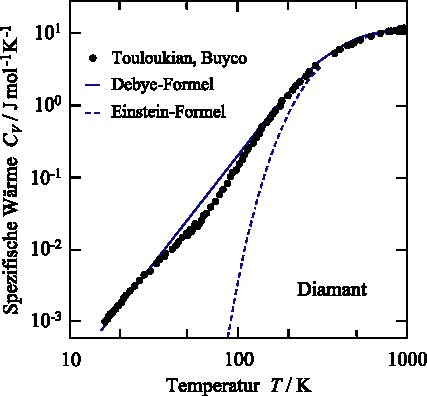
\includegraphics{Bilder/Debye_Einstein.pdf}
  \caption{Spezifische Wärme von Diamant in logarithmischer Darstellung~\cite{Hunklinger}. (Messwerte: Y.S. Touloukian, Thermophysical properties of Matter, Band V)}
  \label{fig:Debye_Einstein}
\end{figure}
% *********************************************
% ***** KAPITEL 4 *****************************
% *********************************************
\newpage
\section{Ergebnisse und Diskussion}\label{sec:ErgebnisseUndDiskussion}

% *********************************************
% ***** KAPITEL 5 *****************************
% *********************************************
\newpage
\section{Zusammenfassung}

% ***** Literaturverzeichnis ******************

\bibliography{Literatur}{}
\bibliographystyle{plain}
\end{document}
